\documentclass[10pt]{beamer}

\usetheme[progressbar=frametitle]{metropolis}
\usepackage{appendixnumberbeamer}

\usepackage{booktabs}
\usepackage[scale=2]{ccicons}

\usepackage{pgfplots}
\usepgfplotslibrary{dateplot}

\usepackage{xspace}
\newcommand{\themename}{\textbf{\textsc{metropolis}}\xspace}

\usepackage{bm}
\usepackage{amsmath,amssymb}
\usepackage{mathtools}

\newcommand{\del}[1]{\ensuremath{\frac{\partial}{\partial #1}}}
\newcommand{\dell}[1]{\ensuremath{\frac{\partial^2}{\partial #1^2}}}

\def\Put(#1,#2)#3{\leavevmode\makebox(0,0){\put(#1,#2){#3}}}


\title{Genetic load and efficacy of selection on admixed populations}
\subtitle{A Diffusion Processes Approach}
% \date{\today}
\date{}
\author{Jonatas Cesar}
\institute{University of S\~ao Paulo \& University of Chicago}
% \titlegraphic{\hfill\includegraphics[height=1.5cm]{logo.pdf}}

\begin{document}

\maketitle

\begin{frame}{Table of contents}
  \setbeamertemplate{section in toc}[sections numbered]
  \tableofcontents[hideallsubsections]
\end{frame}

\section{Genetic Load and Efficacy of Selection}

\begin{frame}{Genetic Load}
  \begin{alertblock}{Definition}
    Genetic load is the relative reduction in the population fitness compared
    to the theoretical "perfectly adapted" genotype.
  \end{alertblock}
  \[
    L = \frac{W_{max} - W}{W_{max}}
  \]
  Causes:
  \begin{itemize}
    \item \underline{Mutation Load}: Influx of new deleterious mutation
    \item Change in environment
    \item Inbreeding 
    \item ...
  \end{itemize}
\end{frame}

\begin{frame}{Equilibrium Rationale}
  \begin{columns}
  \begin{column}{0.65\textwidth}
    \centering
    \begin{footnotesize}
      \begin{tabular}{cccc}
        \\ \hline
        Genotype & aa & aA & AA \\
        Frequency & $(1 - x) ^2$ & $2 x ( 1 - x)$ & $x^2$ \\
        Average Fitness & 1 & $1 - h s$ & $1 - s$ \\
        Mutation Rate & $ a \xrightleftharpoons[u]{v} A $ & \\
        \hline
      \end{tabular}
    \end{footnotesize}
    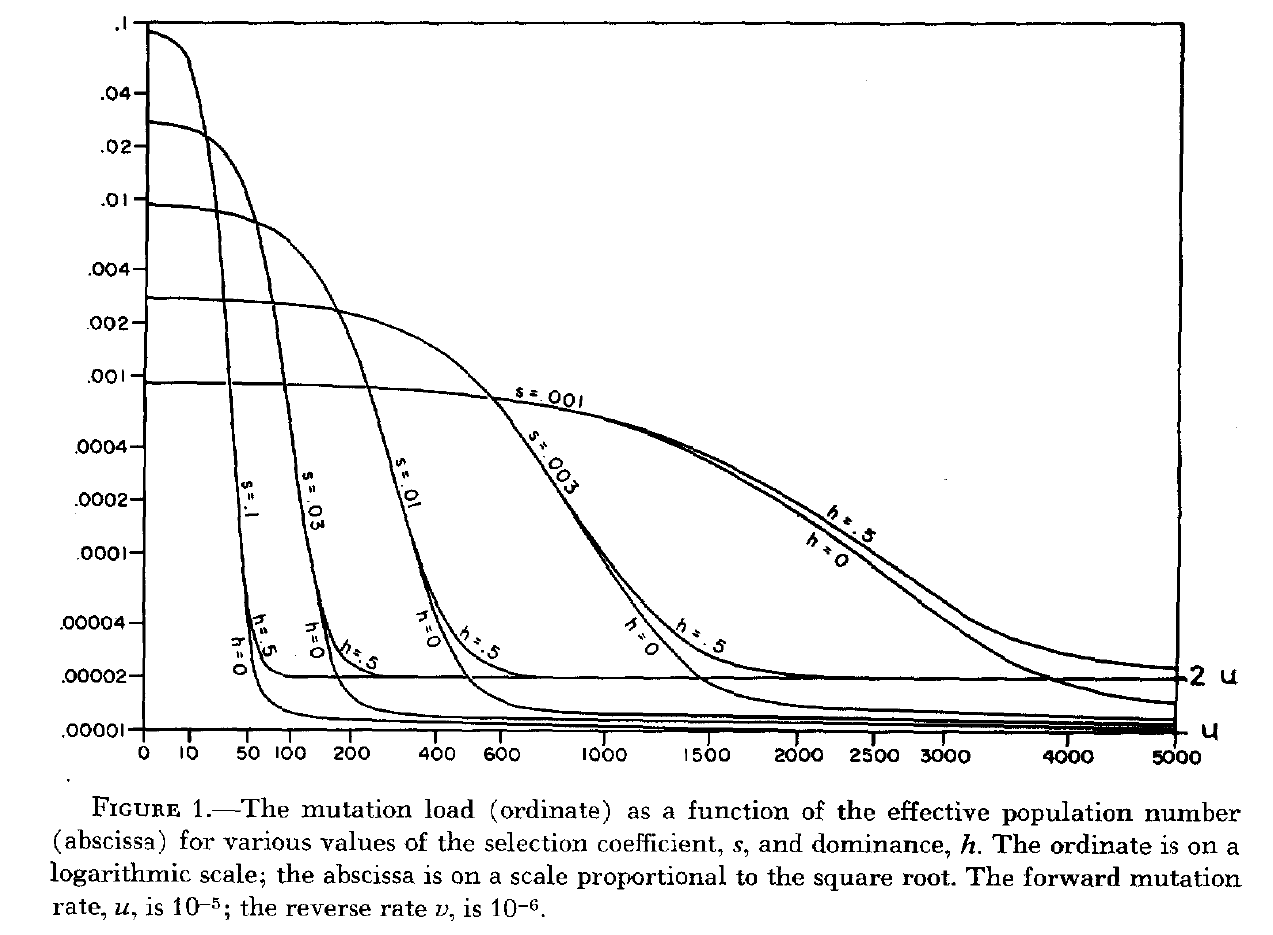
\includegraphics[width=\textwidth]{./Figures/Kimura_1963.png}
  \end{column}
  \begin{column}{0.35\textwidth}
    \begin{scriptsize}
      \begin{tabular}{l}
      Fitness \\ 
      $W(x) = 1 - 2 hs x(1 - x) - s x^2$ \\
      Eq. dist. of $x$ \\ 
      $\phi(x) = C W^{2N} x^{4Nu -1 }(1 - x)^{4Nv - 1}$  \\
      Genetic load \\ 
      $\overline L = \frac{\int_0^1 dx (1 - W)\phi(x)}{\int_0^1 dx \phi(x)}$
      \end{tabular}
    \end{scriptsize}

    \begin{block}{Small Populations}
      Load is high since drift increases the frequency of deleterious
      mutations.
    \end{block}
    \begin{block}{Large Populations}
      Selection decreases the genetic load.\\
      $\overline L \propto u$
    \end{block}
  \end{column}
  \end{columns}
  \let\thefootnote\relax\footnote{
    \scriptsize M. Kimura, T. Maruyama \& J. Crow; The
    Mutation Load in Small Populations. Genetics (1963)}
\end{frame}

\begin{frame}{\normalsize There are differences in mutation load between human
    populations?}
  \vfill
  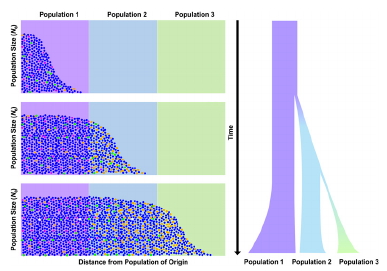
\includegraphics[width=0.8\textwidth]{./Figures/McCoy_Akey2016.png}
  \Put(-50,280){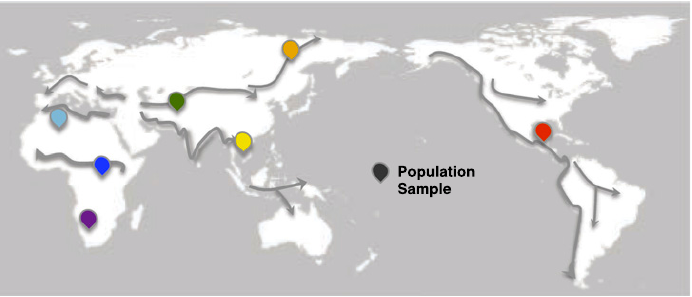
\includegraphics[width=0.4\textwidth]{./Figures/Henn_pnas_map.png}}
  \let\thefootnote\relax\footnote{R. McCoy \& J. Akey, Pnas 2016 \\
    \hspace{3pt} B. Henn, \textit{et.al} Pnas 2016}
\end{frame}

\begin{frame}{It depends}
  \vfill
  \includegraphics[width=\textwidth]{./Figures/Henn_NR_load.pdf}
  \let\thefootnote\relax\footnote{B. Henn \textit{et.al} Nature Review 2016: 
    for snps with GERP 2:4, 4:6 and  $>$6 where assigned $s = -4.5 \times
    10^{-4}$,  $s = -4.5 \times 10^{-3}$ and  $s = -1.0 \times 10^{-1}$ using
    Boyko et al DFE}
\end{frame}

\begin{frame}{\normalsize But there are differences in the present day efficacy
    of selection} 
  \vfill
  \centering
  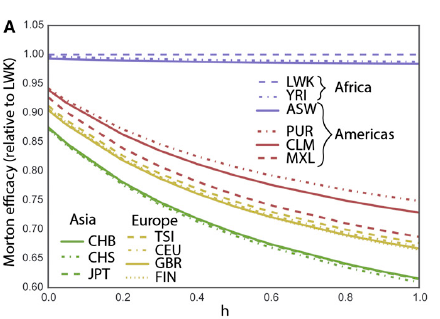
\includegraphics[width=0.8\textwidth]{./Figures/Gravel_efsel.png}
  \let\thefootnote\relax\footnote{S. Gravel, Genetics 2016}
\end{frame}

\begin{frame}{Efficacy of Selection}
  \begin{alertblock}{Definition}
    The efficacy of selection is defined as the contribution of selection on
    the population load change $\partial L / \partial t$.  
  \end{alertblock}
  \begin{block}{Derivation}
    Given the average fitness $W = s[2h\mu_1 + (1 - 2h)\mu_2]$ where
    $\mu_k \equiv \int_0^1 dx x^k \phi(x, t)$ we want to calculate 
    \[
      \frac{d}{dt} W= s[2h \dot \mu_1 + (1 - 2h) \dot \mu_2]
    \]
  \end{block}
  using: 
  $\dot \mu_k = \del t \int_0^1 dx x^k \phi(x, t) = \int_0^1 dx x^k \del t \phi(x, t)$
  \let\thefootnote\relax\footnote{S. Gravel, Genetics 2016}
\end{frame}

\begin{frame}{Derivation outline}
  \begin{alertblock}{Diffusion Approximation}
    Let $\phi(x,t)dx$ the expected number of alleles with frequency between $x$
    and $x + dx$ at time $t$.
    \begin{align}
      \del t \phi(x,t) & \approx \frac{1}{4N} \dell x x(1-x) \phi(x,t) 
      & &\bigg\} \mathrm{drift}
      \nonumber \\ 
      &- s \del x [h + ( 1 - 2h)x]x(1-x) \phi(x,t) 
      & &\bigg\} \mathrm{selection}
      \nonumber \\
      &+ 2Nu\delta\left(x - \frac{1}{2N}\right)
      & &\bigg\} \mathrm{mutation}
    \end{align}
  \end{alertblock}
  \begin{block}{Change in moments ($ k > 0$)}
    \[
      \dot \mu_k = \frac{k(k-1)}{8N} \pi_{k-1} + 
        \frac{sk}{4} \Gamma_{k,h} +
        \frac{u}{(2N)^{k-1}}
    \]
    where $\Gamma_{k,h} = 2[h\pi_k + (1 - 2h) \pi_{k+1}]$ and $\pi_k=(\mu_k - \mu_{k + 1})$
  \end{block}
  \let\thefootnote\relax\footnote{S. Gravel, Genetics 2016}
\end{frame}

\begin{frame}{Single Population Efficacy of Selection}
  \begin{block}{Change in Fitness}
  \begin{align}
    \dot W &= \dot W_u + \dot W_N + \dot W_s
    \nonumber \\
    &= s \big\{
    \underbrace{2hu}_\text{mutation} + 
    \underbrace{\frac{(1 - 2h)\pi_1}{4N}}_\text{drift} + 
    \underbrace{\frac{s}{2}[h\Gamma_{1,h}+(1-2h)\Gamma_{2,h}}_\text{selection}]
      \big\}
  \end{align}
  \end{block}
  \begin{alertblock}{Efficacy of Selection}
  \begin{itemize}
    \item Fit Efficacy (from Fitness increase theorem)
    \[ 
      \dot W_s = \frac{s^2}{2}h\Gamma_{1,h}+(1-2h)\Gamma_{2,h}
    \]

  \item Morton Efficacy (from Morton, Crow and Mueller mutational damage)
    \[ 
      \dot \mu_1 = \frac{s^2}{2}h\Gamma_{1,h}
    \]
  \end{itemize}
  \end{alertblock}

  \let\thefootnote\relax\footnote{where $\Gamma_{k,h} = 2[h\pi_k + (1 - 2h) \pi_{k+1}]$ and $\pi_k=(\mu_k - \mu_{k + 1})$}
\end{frame}

\begin{frame}{\normalsize Efficacy of selection of Admixed populations} 
  \vfill
  \centering
  \[
    \dot W_{s,admix} > \sum_i p_i \dot W_{s,i}
  \]
  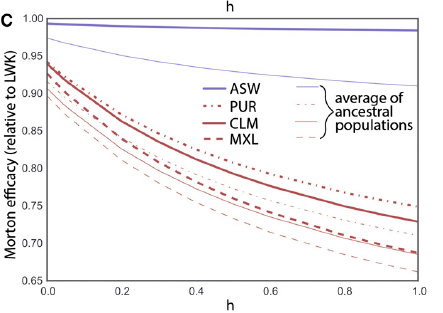
\includegraphics[width=0.8\textwidth]{./Figures/Gravel_efsel_admix.png}
  \let\thefootnote\relax\footnote{S. Gravel, Genetics 2016}
\end{frame}

\begin{frame}{Single Pulse Admixture}

\begin{alertblock}{Allele Frequency Distribution}
  \[
    \phi(x_3) = \int_0^1 \int_0^1 dx_1 dx_2 \phi(x_1, x_2) 
    \delta(x_3 - \alpha_1 x_1 - \alpha_2 x_2) 
  \] 
\end{alertblock}

\begin{block}{Moments of The Admixed Population}
  \begin{align}
    \mu_{3,k} &= \int_0^1 \int_0^1\int_0^1dx_1 dx_2 dx_3 x_3^k \phi(x_1, x_2) 
    \delta(x_3 - \alpha_1 x_1 - \alpha_2 x_2)
    \nonumber \\
    &= \int_0^1 \int_0^1dx_1 dx_2 (\alpha_1 x_1 +  \alpha_2 x_2) ^k \phi(x_1, x_2)
    \nonumber \\
    &= \sum_{j=1}^k\binom{j}{k} \alpha_1^j\alpha_2^{k -j} 
    \int_0^1 \int_0^1dx_1 dx_2 x_1^jx_2^{k -j} \phi(x_1, x_2)
    \nonumber \\
    &= \sum_{j=1}^k\binom{j}{k} \alpha_1^j\alpha_2^{k -j} 
    \mu_{j,k-j}^{1,2}
  \end{align}
\end{block}
  
\end{frame}

\begin{frame}{\normalsize Present day efficacy
    of selection - CADD $>$ 2} 
  \vfill
  \centering
  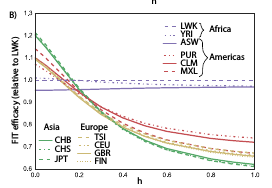
\includegraphics[width=0.8\textwidth]{./Figures/Gravel_efsel_CADD.png}
  \let\thefootnote\relax\footnote{S. Gravel, Genetics 2016}
\end{frame}

\section{Diffusion simulation}
\begin{frame}[t]{Out of Africa Simulation}
  \vfill
  \centering
  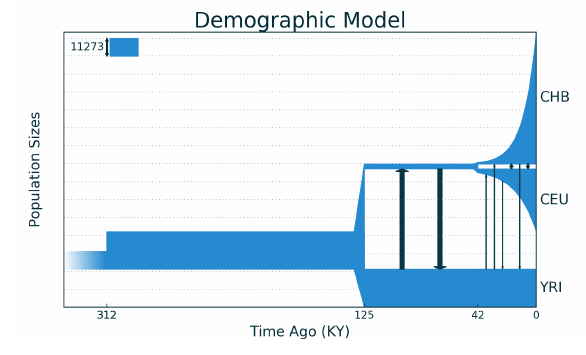
\includegraphics[width=0.8\textwidth]{./Figures/moments_simul.png}
  \let\thefootnote\relax\footnote{Jouganous, Genetics 2017}
\end{frame}

\begin{frame}[t]{Genetic Load}
  \vfill
  \centering
  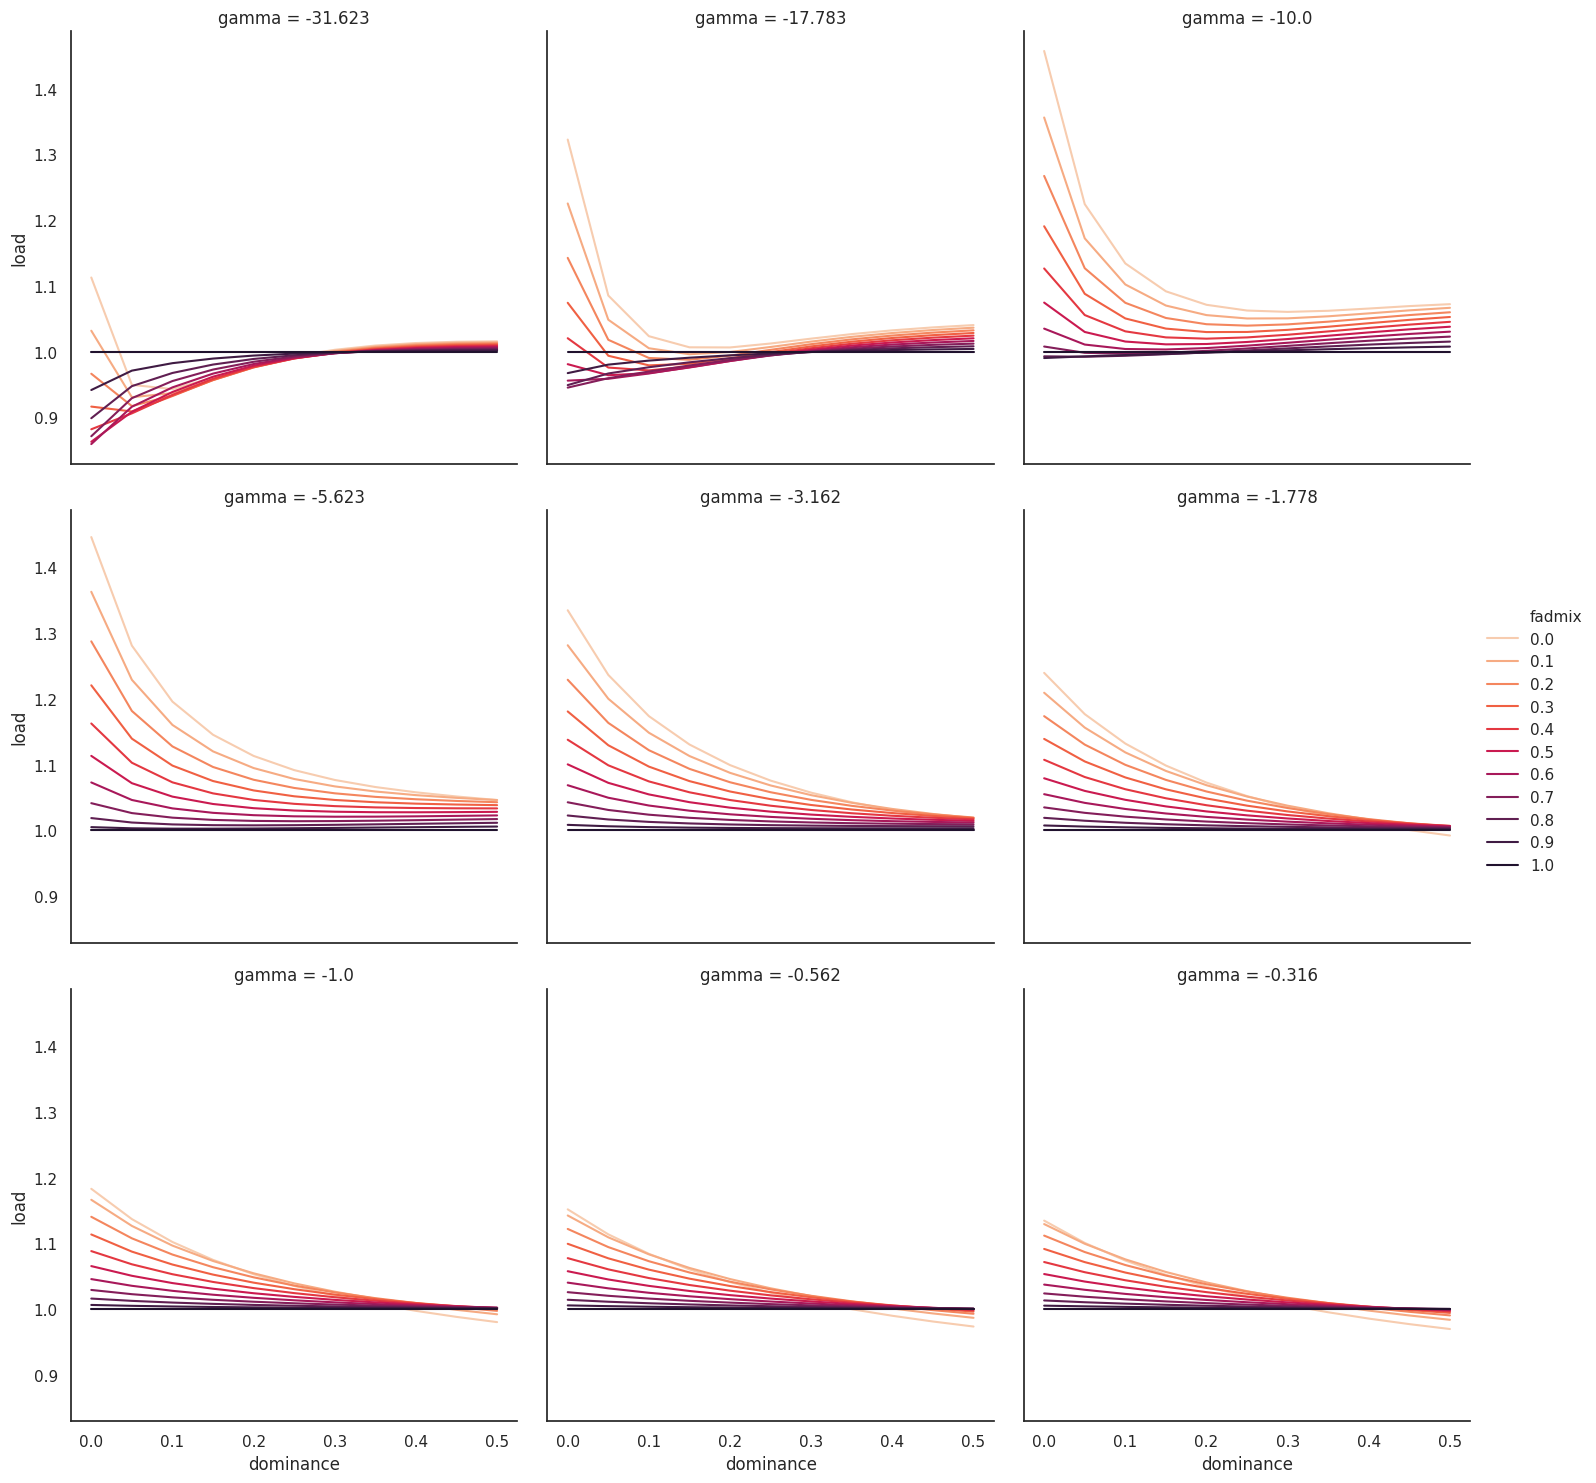
\includegraphics[width=0.8\textwidth]{./Figures/load.png}
\end{frame}

\begin{frame}[t]{Number of deleterious mutations}
  \vfill
  \centering
  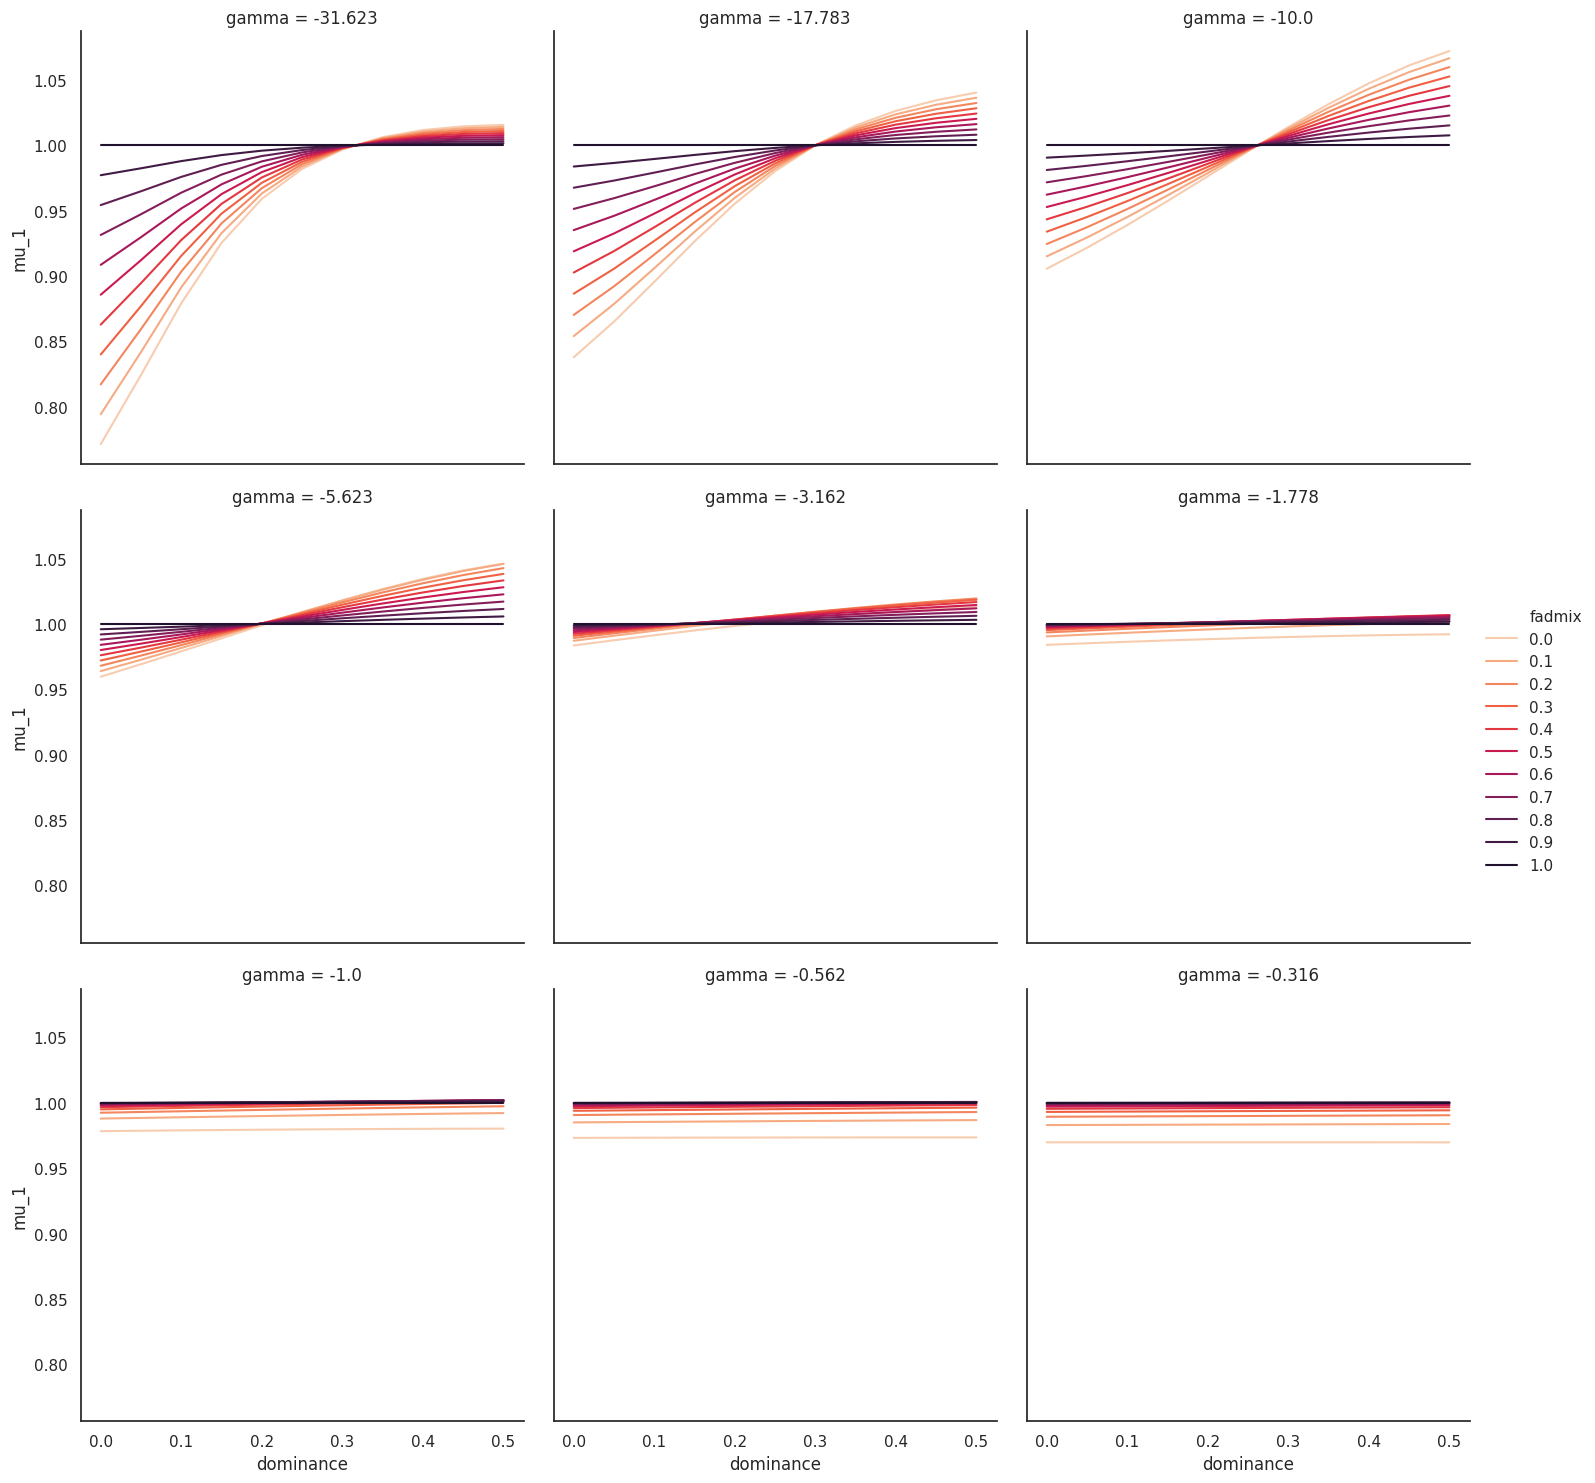
\includegraphics[width=0.8\textwidth]{./Figures/mu_1.png}
\end{frame}

\begin{frame}[t]{Nucleotide diversity}
  \vfill
  \centering
  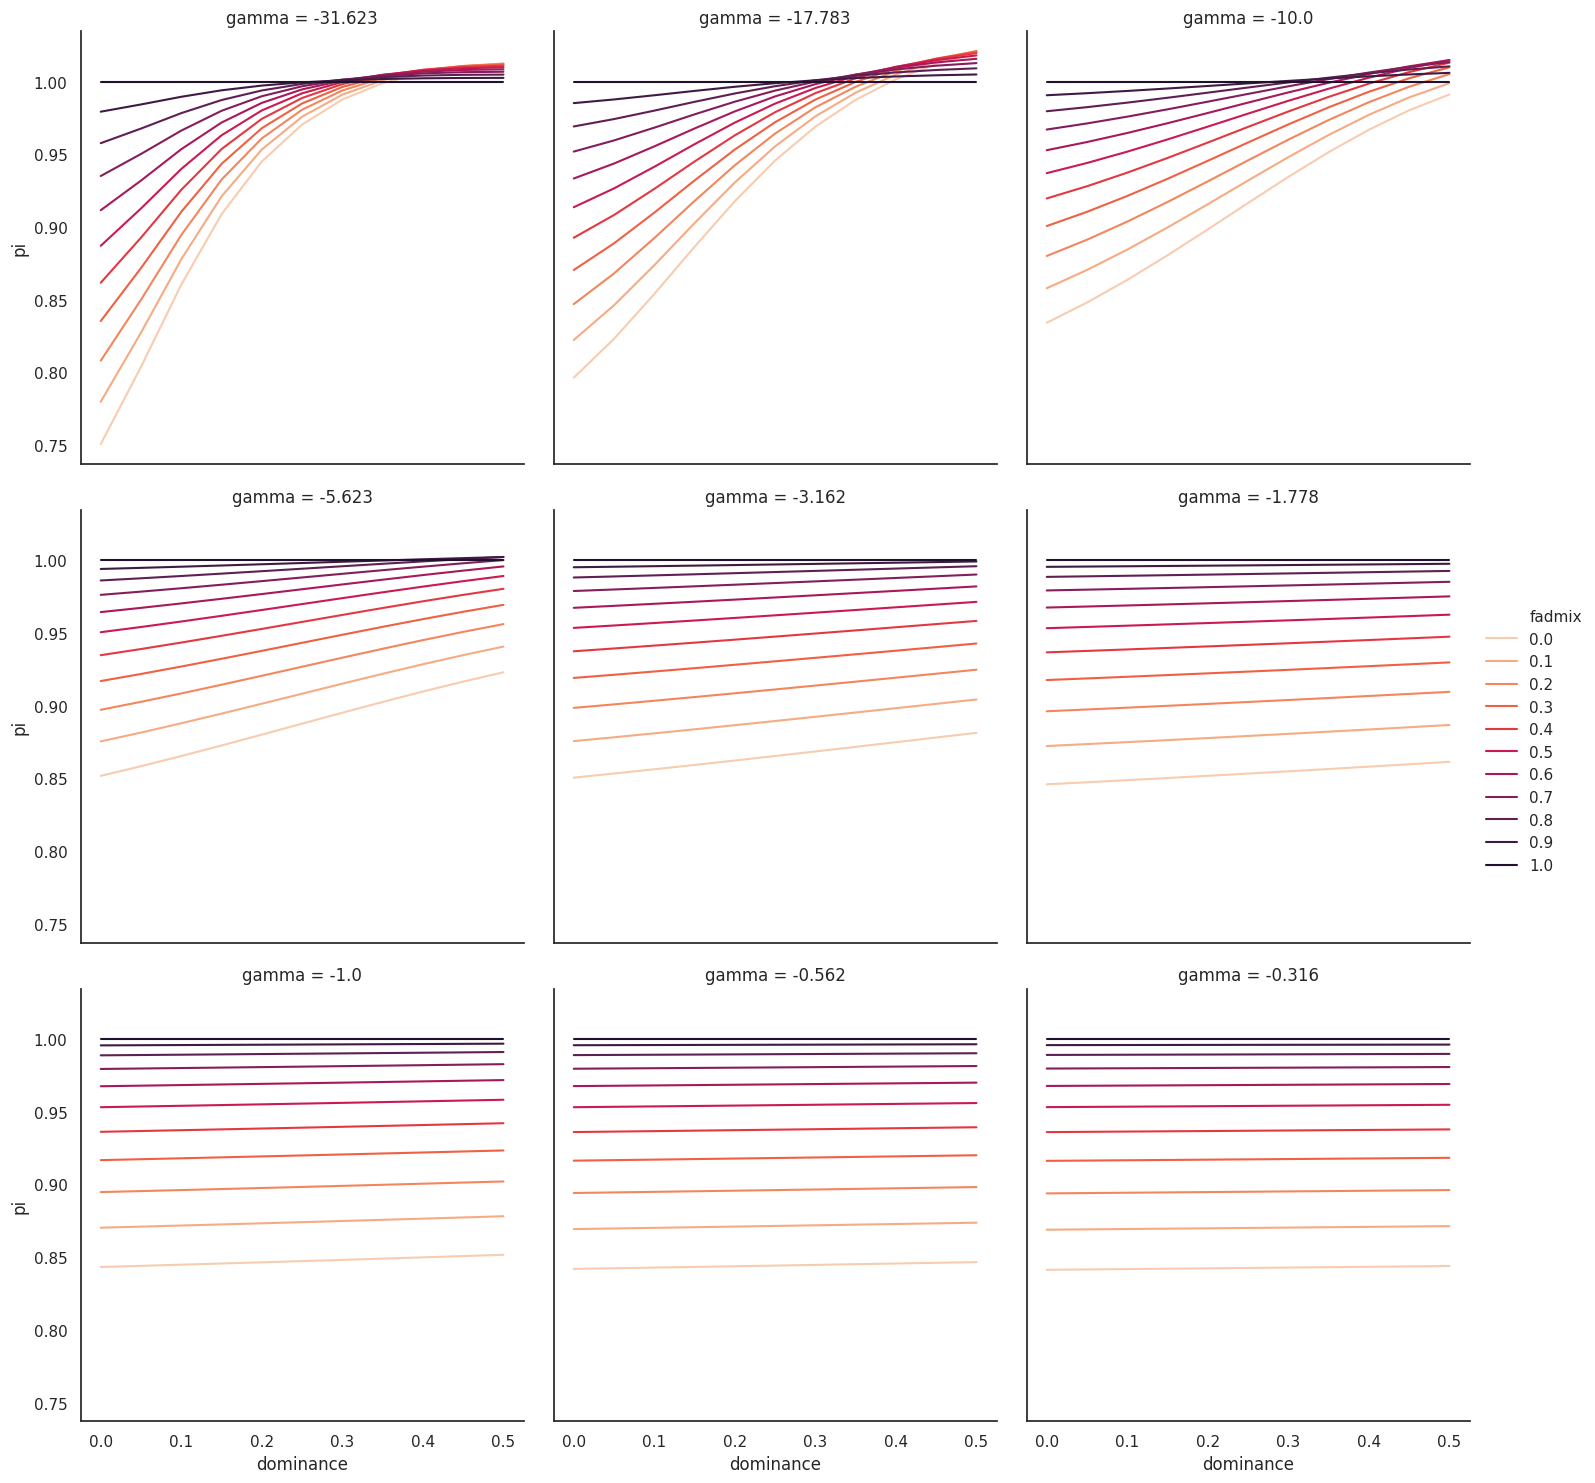
\includegraphics[width=0.8\textwidth]{./Figures/pi.png}
\end{frame}


\begin{frame}[t]{Fit efficacy}
  \vfill
  \centering
  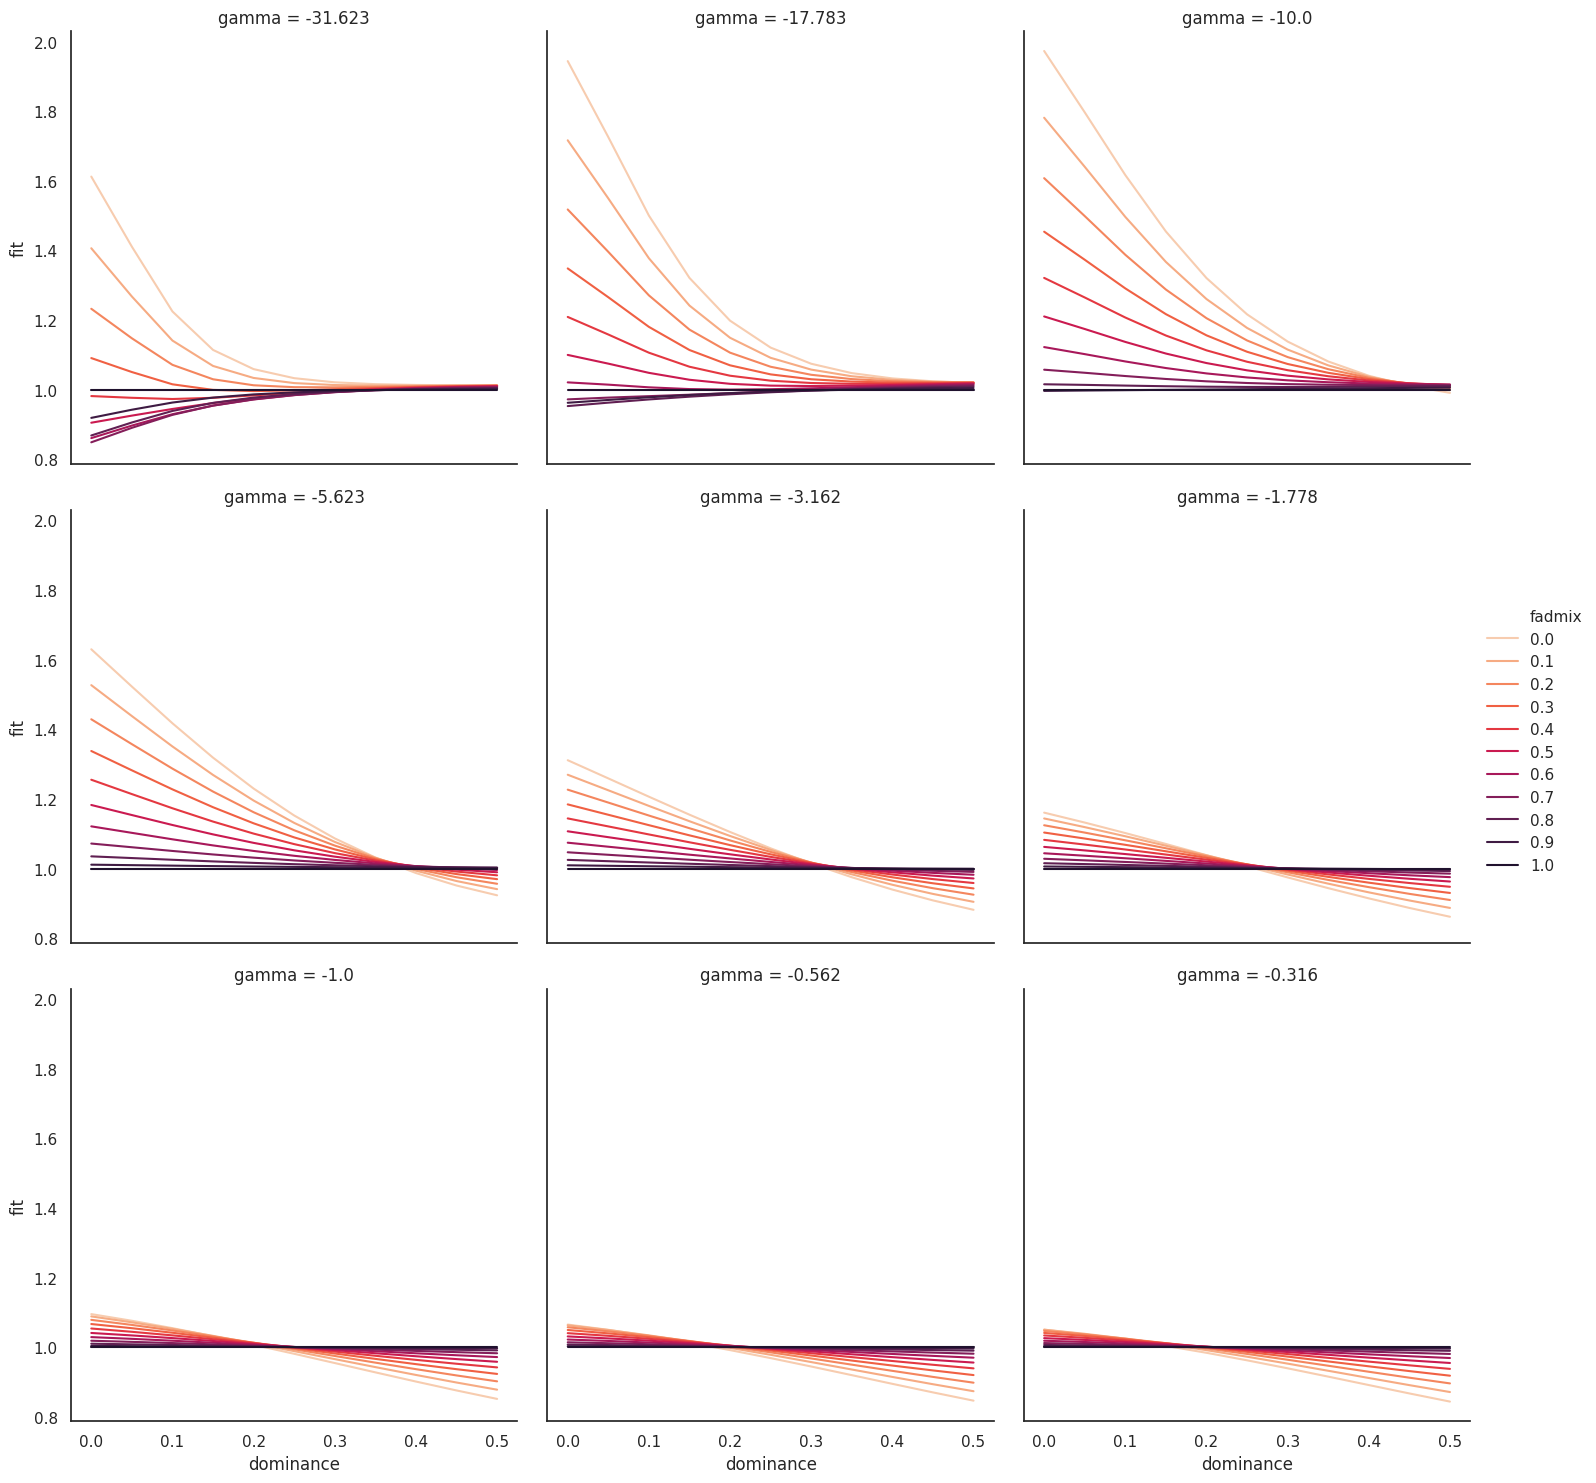
\includegraphics[width=0.8\textwidth]{./Figures/fit.png}
\end{frame}


\begin{frame}[t]{Morton Efficacy}
  \vfill
  \centering
  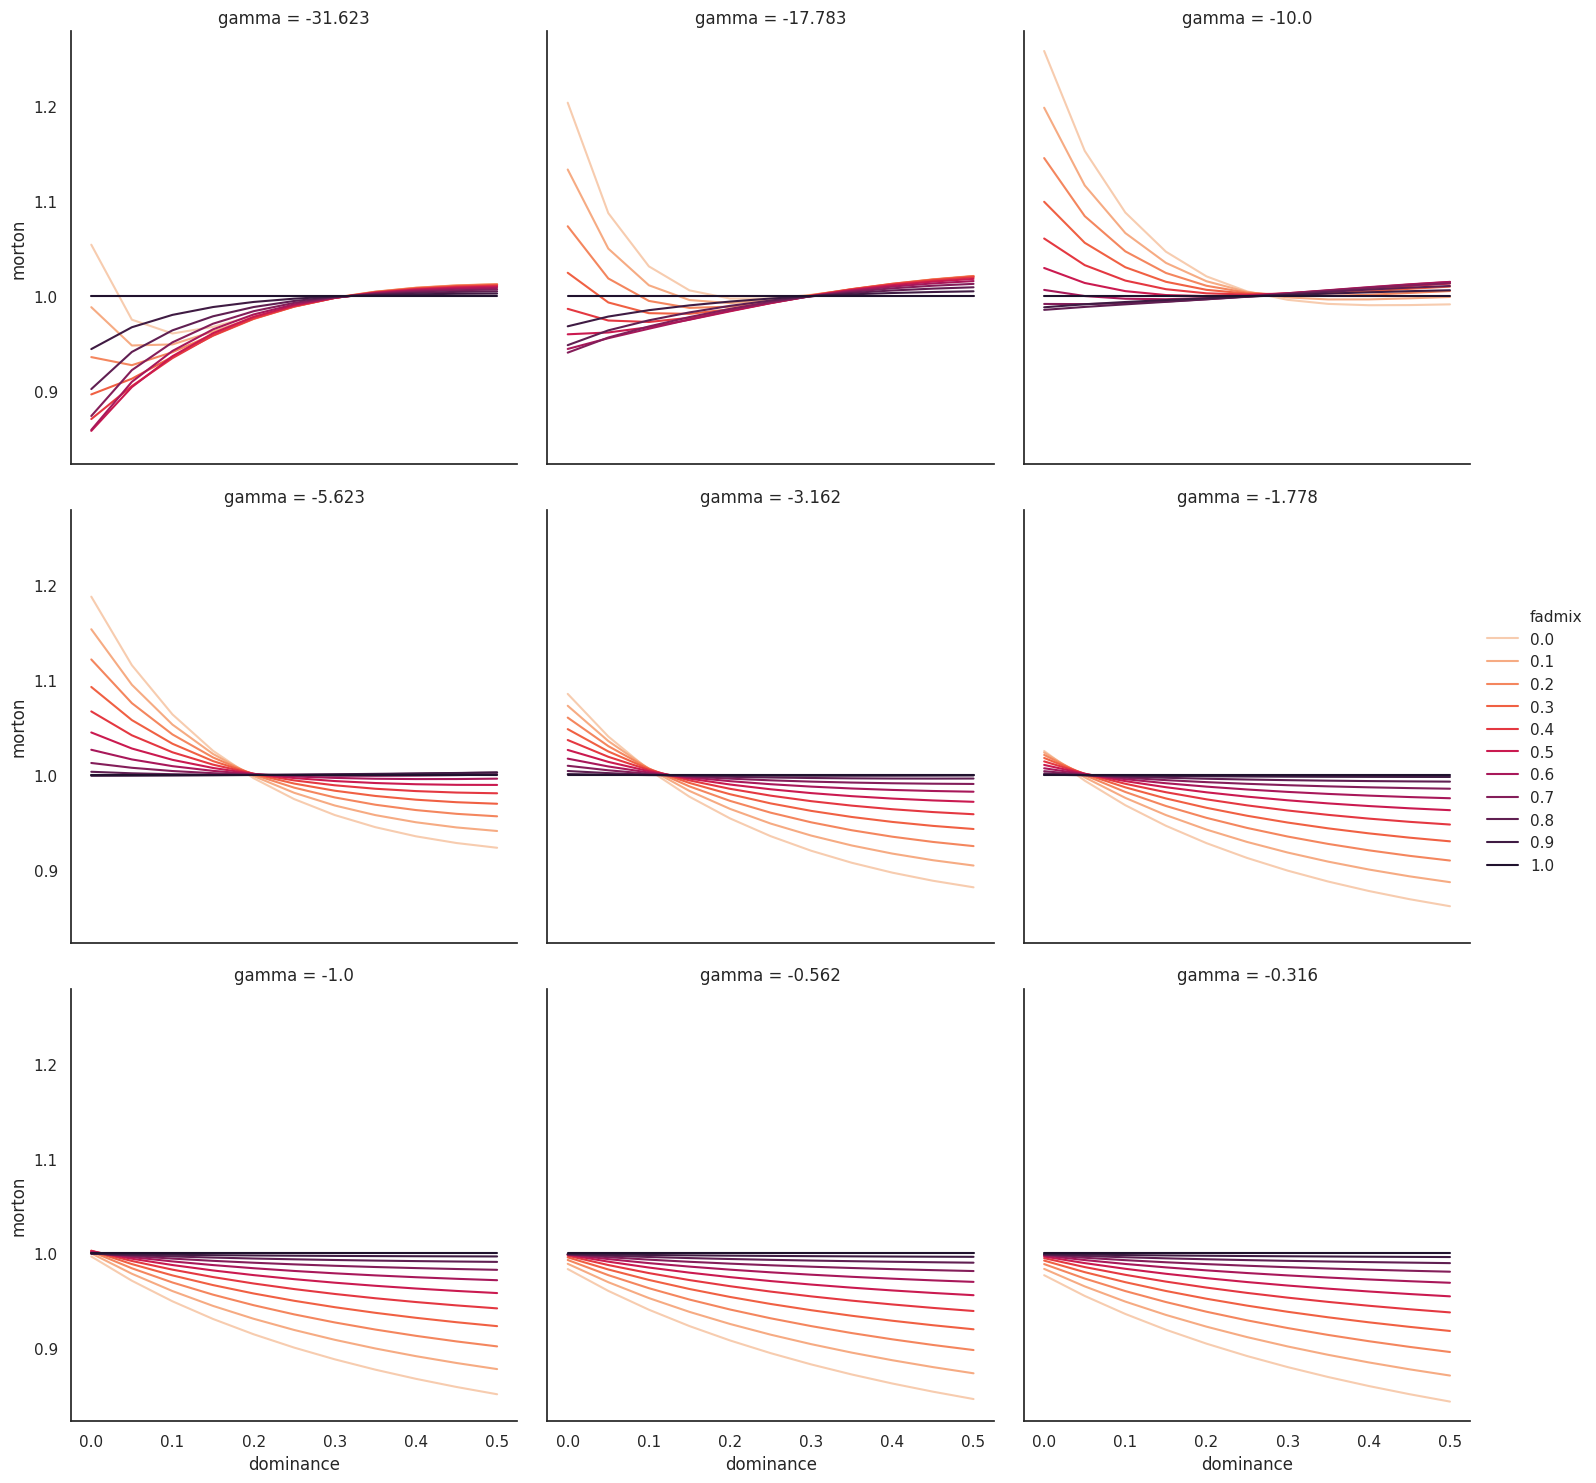
\includegraphics[width=0.8\textwidth]{./Figures/morton.png}
\end{frame}

\section{Further Steps}

\begin{frame}[t]{From near to not so near future}
  \begin{itemize}
    \item More realistic simulations with Slim3
      \begin{itemize}
        \item Recombination
        \item Distribution of Fitness Effects
        \item Dominance models
      \end{itemize}
    \item Real data analysis
      \begin{itemize}
        \item 1000G 
        \item GnomAD 
        \item AbraOM (1.2K Brazilians)
      \end{itemize}
    \item Impact of dominance and admixture on GWAS
      \begin{itemize}
        \item Eyre-Walker (2010)   
        \item Simons (2017)
      \end{itemize}
  \end{itemize}
\end{frame}

\end{document}
